\newpage
\section{Process modeling}
\subsection{Process components}
Operator -> Equipment <-> Material-> Part


A Manufacturing Process is a Changein the Workpiece Material
•A change in geometry
•A change in constitutive properties

There is an energy transfer occurring: mechanical, electrical, thermal or chemical 


\subsubsection{Variability}
Control of variation: identify, characterize, minimize.

Deterministic
Random: measure with probability, statistics, predict

Manufacturing: Quality, Rate, Cost, Flexibility
Quality: conformance to specifications => minimize variability

Deterministic: equipment, material, operation
Random: probabilistic model of the process, Statistics as output, Deviation from expected behaviour
Variation reduction, factors influencing statistical behaviour, optimization of statistical behavior
Sources: material, equipment, operator and environment

\begin{table}[!htb]
	\centering
    \def\arraystretch{1.5}
		\begin{tabular}{l l l}
	 \hline
      & States & Properties \\
	  \hline
		Material & & \\
		
		Equipment & & 
		\end{tabular}
	\caption{Process Parameters}
	\label{tab:bezeichnungen}
\end{table}

\begin{equation}
\Delta Y=\frac{\partial Y}{\partial \alpha}\Delta \alpha + \frac{\partial Y}{\partial u}\Delta u 
\end{equation}

With $\frac{\partial Y}{\partial \alpha}$ Disturbance Sensitivity, $\Delta \alpha$ Disturbances, $\frac{\partial Y}{\partial u}$ Control Sensitivity and $\Delta u$ Control Inputs.

Disturbances are reduced with standard operating procedures (SOPs) and Statistical analysis and identification of variation sources (SPC). The sensitivity of the disturbances are reduces with designed experiments to measure the sensitivity and thus make the process robust. Finally the more direct approach is to measure the output and manipulate the input with the so-called feedback control. Here under are schematically depicted the three methods 

\begin{figure}[h]
\centering
  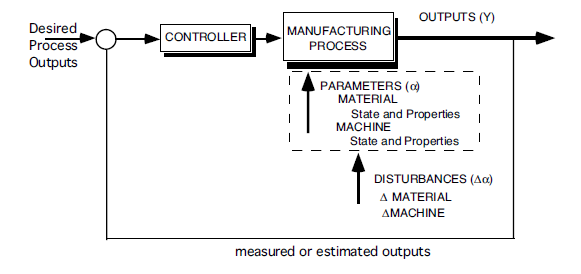
\includegraphics[height=4cm]{img/directfb.PNG}
   \caption{adaptive mesh generation}
 \label{fgr:graft}
\end{figure}





\begin{enumerate}
\item Physical Model
\item Empirical Model
\item Statistical Model
\end{enumerate}


Variation Equation
Reduce Disturbances (Statistical Analysis)
Reduce Senstivity (optimization \& robustness)


 Design, Optimization and Robustness Analysis

\subsection{Experimental design}
\subsubsection{ANOVA}
\subsubsection{Design of Experiments (DoE)}
Correlation
Regression
Full Factorial
Taguchi


\subsection{Metamodeling}
Study Physics of Process
–Define Important Inputs
–Intuition about model
–Limits on inputs
•Define Optimization Penalty Function
–J=f(x)


Procedure
•Identify model (linear, quadratic, terms to include)
•Define inputs and ranges
•Identify “noise”parameters to vary if possible ($\Delta \alpha$’s)
•Perform Experiment
–Appropriate order
•randomization
•blocking against nuisance or confounding effects


Solve for $\beta$’s
•Apply ANOVA
–Data significant?
–Terms significant?
–Lack of Fit Significant?
•Drop Insignificant Terms
•Add Higher Order Terms as needed
Search for Optimum
–Analytically
–Piecewise
–Continuously
Find Optimum value x*
•Perform Confirming experiment
–Test Model at x*
–Evaluate error with respect to model
–Test hypothesis that
y(x*)=ˆ y (x*)
If hypothesis fails
–Consider new ranges for inputs
–Consider higher order model as needed
–Boundary may be optimum!

Procedure for DOE/OptimizationFor

Study Physics of Process–Define important inputs–Intuition about model–Limits on inputs•DOE–Factor screening experiments–Further DOE as needed–RSM Construction•Define Optimization/Penalty Function–J=f(x)


(1) DOE Procedure


•Identify model (linear, quadratic, terms to include)
•Define inputs and ranges
•Identify “noise”parameters to vary if possible ($\Delta \alpha$’s)
•Perform experiment
–Appropriate order
•randomization
•blocking against nuisance or confounding effects

(2) RSM Procedure


•Solve for $\beta$’s
•Apply ANOVA
–Data significant?
–Terms significant?
–Lack of Fit significant?
•Drop Insignificant Terms
•Add Higher Order Terms as needed


(3) Optimization Procedure


•Define Optimization/Penalty Function
•Search for Optimum
–Analytically
–Piecewise
–Continuously/evolutionary
•Confirm Optimum


